\documentclass{beamer}
\setbeamertemplate{navigation symbols}{}
\usepackage{xcolor}
\definecolor{seeblau}{HTML}{00A9E0}
\definecolor{seegrau}{HTML}{9AA0A7}

\definecolor{seeblau1}{HTML}{CCEEF9}
\definecolor{seeblau2}{HTML}{A6E1F4}
\definecolor{seeblau3}{HTML}{59C7EB}
\definecolor{seeblau4}{HTML}{00A9E0}
\definecolor{seeblau5}{HTML}{008ECE}

\setbeamercolor{title}{fg=seeblau}
\setbeamercolor{frametitle}{fg=seeblau}
\setbeamercolor{section in toc}{fg=seeblau}
\setbeamercolor{structure}{fg=seeblau}

\setbeamertemplate{footline}{%
	\begin{beamercolorbox}[sep=.25cm,wd=\paperwidth,leftskip=0.25cm,rightskip=0.25cm]{footlinecolor}
		\small
		% \textbf{\insertsection}\quad\insertsubsection
		% \hfill\insertframenumber
	\end{beamercolorbox}%
}

\usepackage[overridenote]{pdfpc}

\usepackage[english]{babel}
\parskip=20pt

\usepackage[sfdefault]{roboto}
\usepackage{libertinust1math}
\usefonttheme[onlymath]{serif}

\usepackage{ifthen, adjustbox}
\newcommand{\markieren}[4]{
	\ifthenelse{\equal{#1}{}}{}{\adjustbox{padding=3pt, bgcolor=seeblau1, margin=-1pt}{\strut{\sffamily\robotoMedium{#1}}}\\}
  \ifthenelse{\equal{#2}{}}{}{\adjustbox{padding=3pt, bgcolor=seeblau2, margin=-1pt}{\strut{\sffamily\robotoMedium{#2}}}\\}
	\ifthenelse{\equal{#3}{}}{}{\adjustbox{padding=3pt, bgcolor=seeblau3, margin=-1pt}{\strut{\sffamily\robotoMedium{#3}}}\\}
	\ifthenelse{\equal{#4}{}}{}{\adjustbox{padding=3pt, bgcolor=seeblau4, margin=-1pt}{\strut{\sffamily\robotoMedium{#4}}}}
}

\let\footnoterule\relax % removes bar
\setbeamertemplate{footnote}{
  \parindent 0em\noindent
  \raggedleft
  \usebeamercolor{footnote}\hbox to 0.8em{\hfil\insertfootnotemark}\tiny\insertfootnotetext\par%
}

\newcommand\blfootnote[1]{
	\let\thefootnote\relax\footnotetext{#1}
}

\usepackage[
	style=authortitle
]{biblatex}
\usepackage{ifthen}
\newcommand{\customcite}[2][]{
	\blfootnote{
		\emph{\citetitle{#2}}, \citeauthor*{#2} \citeyear{#2}
		\ifthenelse{ \equal{#1}{} }{}{(#1)}
	}
}


\usepackage[ddmmyyyy]{datetime}
\renewcommand{\dateseparator}{.}

\usepackage{amsmath,amssymb,amsfonts,amsthm}

\addbibresource{literature.bib} 
\DeclareMathOperator{\Tr}{Tr}

\title{Noise Analysis in an Optomechanical Resonance Cavity}
\author{Leon Oleschko}
\institute{Universität Konstanz}
\date{\today}

\begin{document}
{
\setbeamertemplate{footline}{} 
\begin{frame}
	\huge
	\markieren{}{}{Noise Analysis}{Optomechanical Cavity}
	
	\vfill
	\normalsize
	Leon Oleschko\\
	\today
	
	\vfill
	\raggedleft
	\small
	\textit{Modeling Quantum Hardware: open dynamics and control}\\
	Universität Konstanz
\end{frame}
}



\section{Strong Measurement}
\begin{frame}{Strong Measurement}
	Projective Measurement:
	
	\customcite[2.2.3]{nielsen_quantum_2010}
\end{frame}

\begin{frame}{Qbit System}
	\begin{align*}
		H &= \sigma_x\\
		C &= \sigma_z
	\end{align*}	
\end{frame}

\begin{frame}{Measurement}
	\begin{center}
		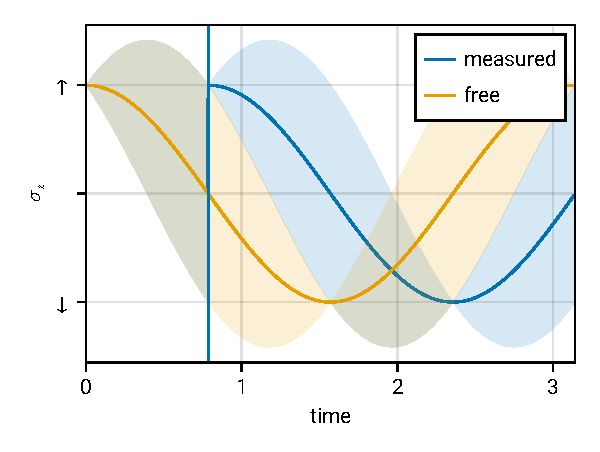
\includegraphics{figures/03 measurement.pdf}
	\end{center}
\end{frame}

\begin{frame}{Discrete Zeno}
	\begin{center}
		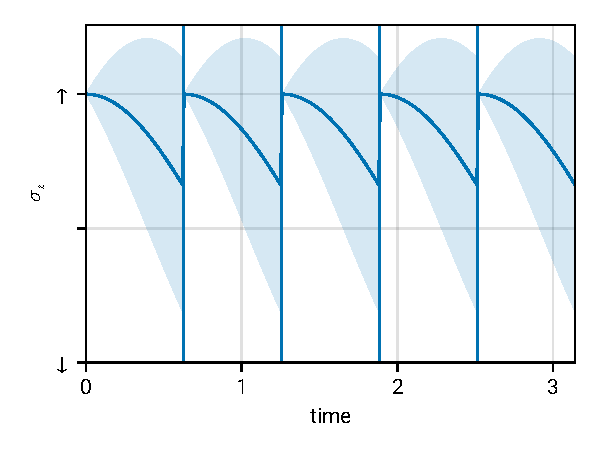
\includegraphics{figures/04 discreate zeno.pdf}
	\end{center}
\end{frame}


\section{Weak Measurement}
\begin{frame}{Weak Measurement}
	\begin{center}
		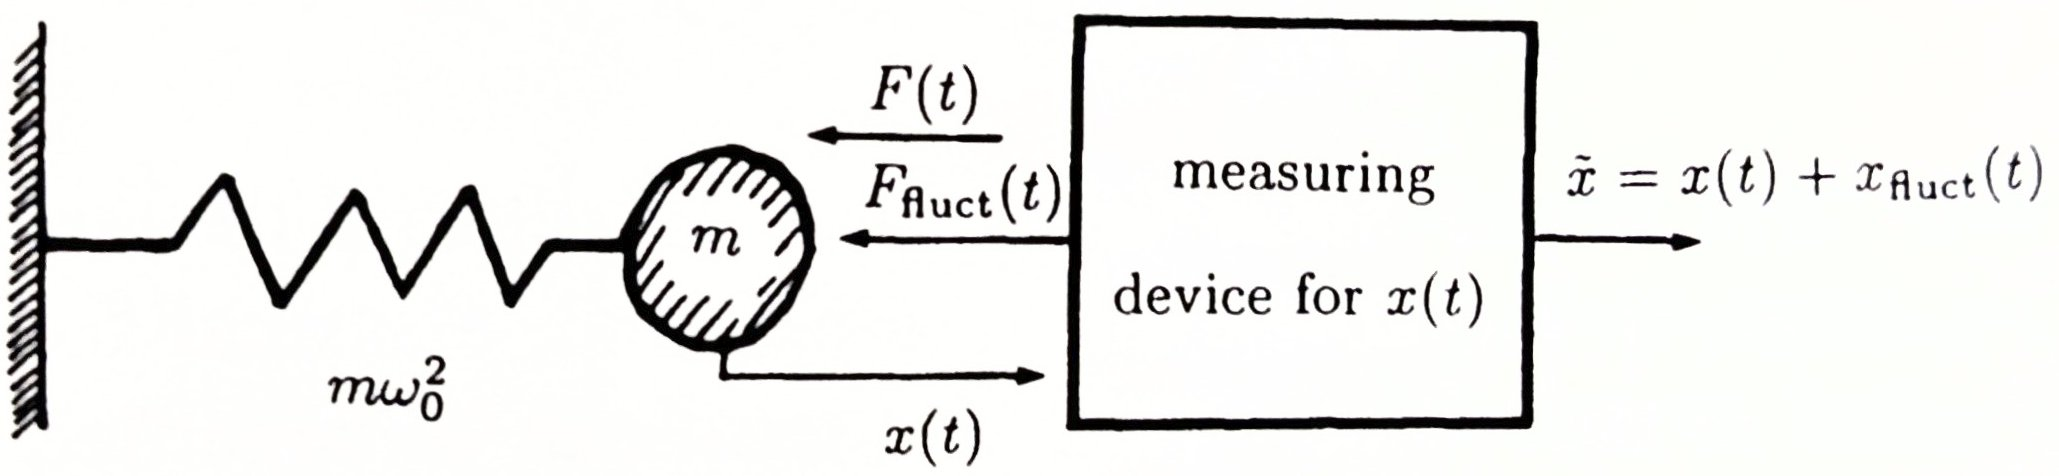
\includegraphics[width=\textwidth]{figures/Fig. 8.4.jpg}
	\end{center}
	\customcite[]{vladimir_braginsky_quantum_1992}
\end{frame}

\begin{frame}{Rabi Oscillations Setup}
	\begin{columns}
		\column{.5\textwidth}
		\begin{center}
			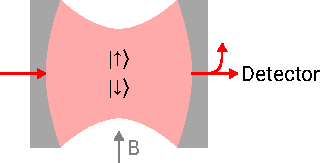
\includegraphics{figures/rabi.pdf}
		\end{center}

		\column{.5\textwidth}
		\begin{align*}
			H &= g\; (a^\dagger a) (\sigma^+ \sigma^-) &\text{Coupling}\\
			&+ g_s\; (\sigma^+ + \sigma^-) &\text{Magnetic}\\
			&- i \beta (a^\dagger - a) &\text{Optic}\\
			J &= \kappa\; a &\text{Dissipation}\\
			C &= \sqrt{\kappa\eta}\; a &\text{Measurement}
		\end{align*}
		
	\end{columns}

	\customcite{nielsen_stochastic_2008}
\end{frame}

\begin{frame}{Time evolution}
	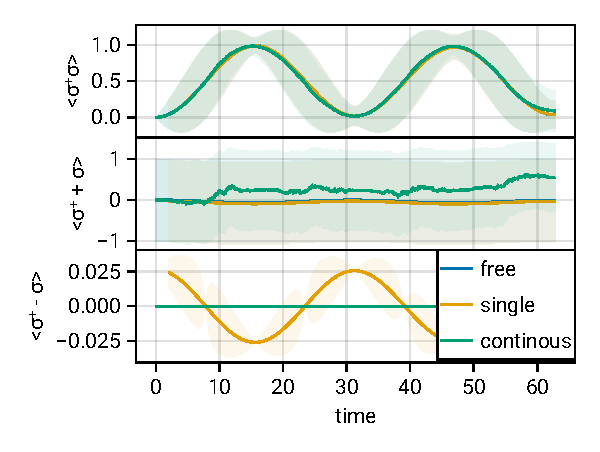
\includegraphics{figures/02 rabi w measurement.pdf}
\end{frame}


{
	\setbeamercolor{background canvas}{bg=black}
	\begin{frame}[plain]{}\end{frame}
}

\section{Appendix}
% \section{Problem Statement}
\begin{frame}{Problem Statement}
	\begin{columns}
		\column{0.5\textwidth}
		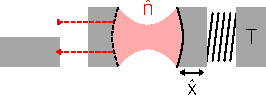
\includegraphics[width=\textwidth]{figures/drawing.pdf}

	\end{columns}

	\customcite{aspelmeyer_cavity_2014}
	\customcite{bowen_quantum_2015}
\end{frame}

\begin{frame}{Hamiltonian}

	{
		\small
		Optical Cavity $\hat a$, $\omega_o(\hat x_\text{mech}) = \omega_o + \frac{g}{\omega_o} \hat x_\text{mech}$;
		mechanical oscillations $\hat b, \omega_m$;
		coupling $g$;
		Drive $E$, $\omega_L$
		\blfootnote{$\hbar=1$}
	}
	$$
		H = \underbrace{
			\omega_o\; a^\dagger a
		}_\text{Cavity} 
		+ \underbrace{
			\omega_m\; b^\dagger b
		}_\text{Mechanical}
		- \underbrace{
			g\; a^\dagger a\; (b + b^\dagger)
		}_{\text{Interaction}}
		+ \underbrace{
			E ( a e^{i\omega_L t} + a^\dagger e^{-i\omega_L t} )
		}_{\text{Drive}}
	$$

	\emph{Rotating Wave Approximation} at $\omega_L$ with $\Delta = \omega_o - \omega_L$, $a \rightarrow ae^{i\omega_L t}$:
	$$
		H_\text{RWA} = \Delta\; a^\dagger a + \omega_m\; b^\dagger b - g\; a^\dagger a\; (b^\dagger + b) 
		+ E ( a + a^\dagger)
	$$

	\customcite[2.3]{bowen_quantum_2015}
	\customcite[Optomechanical Cavity]{kramer_quantumopticsjl_2024}
\end{frame}

\begin{frame}{Hamiltonian Linearization (Currently not used)}
	\textcolor{seegrau}{
		$$
			H_\text{RWA} = \Delta\; a^\dagger a + \omega_m\; b^\dagger b - g\; a^\dagger a\; (b^\dagger + b) 
			+ E (a+ a^\dagger)
		$$
	}	

	Linearize $a = \alpha + \delta a$, $b = \beta + \delta b$; with $\alpha, \beta$ steady state.\\
	\begin{align*}
		H_\text{Interaction} &= 
		- g\; a^\dagger a\; (b^\dagger + b)\\
		&\approx -\underbrace{g |\alpha|}_{G} 
		\left(\delta a + \delta a^\dagger + \textcolor{seegrau}{\mathcal{O}(a^2 + \delta a \delta a^\dagger) }\right)
		\left(\delta b + \delta b^\dagger + \textcolor{seegrau}{2 \beta}\right)\\
		a + a^\dagger
		&= |\alpha| + \delta a + \delta a^\dagger
		\sim \delta a + \delta a^\dagger
	\end{align*}

	Therefore for small $G$:
	\begin{align*}
		H_\text{lin} &= \Delta\; \delta a^\dagger \delta a 
		+ \omega_m \delta b^\dagger \delta b
		- G (\delta a + \delta a^\dagger)(\delta b + \delta b^\dagger)
		+ E(a+a^\dagger)
		\\
		&\sim \frac{\Delta}{2} (\hat X^2 + \hat Y^2) + \frac{\omega}{2} (\hat Q^2 + \hat P^2) - G \hat X \hat Q 
		+ E \hat X
	\end{align*}

	\customcite[2.7]{bowen_quantum_2015}
\end{frame}

\begin{frame}{Linearization in Quadratures}
	$X = \delta a + \delta a^\dagger$\quad
	$Q = \delta b + \delta b^\dagger$\\
	$Y = i(\delta a^\dagger - \delta a)$\quad
	$P = i(\delta b^\dagger - \delta b)$\\
	$n = \delta a^\dagger a$\quad
	$m = \delta b^\dagger b$
	\begin{align*}
		H_\text{RWA} &= \Delta n + \omega m - g n Q + E X\\
		H_\text{lin} &= \Delta n + \omega m - G X Q + E X\\
	\end{align*}

	\small
	The drive $EX$ is not getting lost in linearization.\\
	There is no point in the simplification if solved numerically.
\end{frame}

\begin{frame}{Dissipation}
	Optical decay $\kappa$:
	$$L = \sqrt{\kappa (n_T+1)} \;\delta a 
		+ \sqrt{\kappa n_T} \; \delta a^\dagger$$
	
	Mechanical resonator with $\gamma$ and a thermal bath at the $n$-th thermal state:
	$$
		+ \sqrt{\gamma (m_T+1)} \;\delta b 
		+ \sqrt{\gamma m_T} \; \delta b^\dagger
	$$
	\customcite[2.8]{bowen_quantum_2015}
\end{frame}

\section{Implementation}
\begin{frame}{Implementation}
truncated Fock Basis: $F_\text{optical} \otimes F_\text{mechanical}$

definition of $H, J$ with $\delta a \otimes 1$

$\psi(0) = |0\rangle \otimes |0\rangle$

Time Evolution using the \emph{Lindblad equation}: 
$$
	\dot\rho = -i[H,\rho] + J\rho J^\dagger - \frac{1}{2} \{J^\dagger J, \rho\}
$$
\customcite{kramer_quantumopticsjl_2024}
\end{frame}

\section{Measurement}
\begin{frame}{Continous measurement}
	\textcolor{seegrau}{
		Lindblad Master Equation:
		$$\dot\rho = -i[H,\rho] + J\rho J^\dagger - \frac{1}{2} \{J^\dagger J, \rho\}$$
	}

	Stochastic Master Equation:
	$$
		\dot\rho 
		= -i[H,\rho] 
		+ J\rho J^\dagger - \frac{1}{2} \{J^\dagger J, \rho\} 
		+ \left(C\rho + \rho C^\dagger - \Tr(C\rho + \rho C^\dagger)\right)\xi(t)
	$$

	Let's look at the Quadrature $C = \eta\sqrt{\kappa}\;(\delta a + \delta a^\dagger)$

	\customcite[Stochastic Master equation, Quantum Zeno Effect]{kramer_quantumopticsjl_2024}
	\customcite{jacobs_straightforward_2006}
\end{frame}

\begin{frame}{Time Evolution}
	\centering
	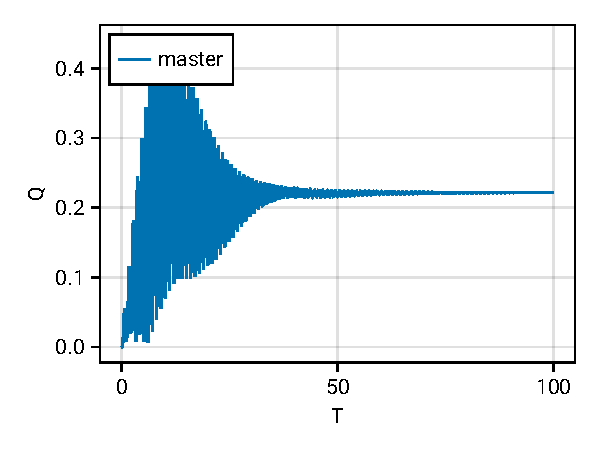
\includegraphics{figures/01 time evolution.pdf}
\end{frame}

\begin{frame}{Spectrum}
	\centering
	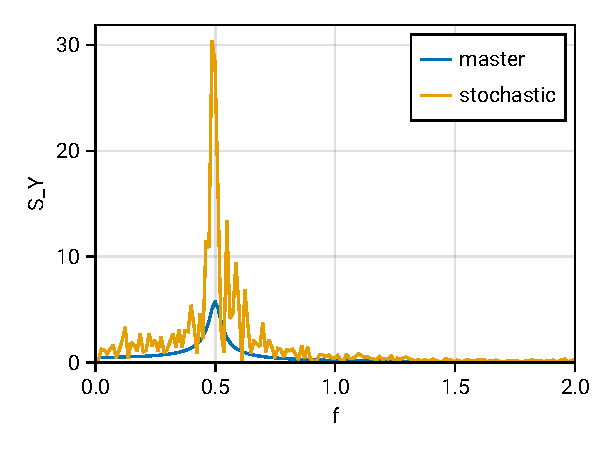
\includegraphics{figures/01 time evolution spectrum.pdf}
\end{frame}

\begin{frame}{Power Dependence $\sim$ G}
	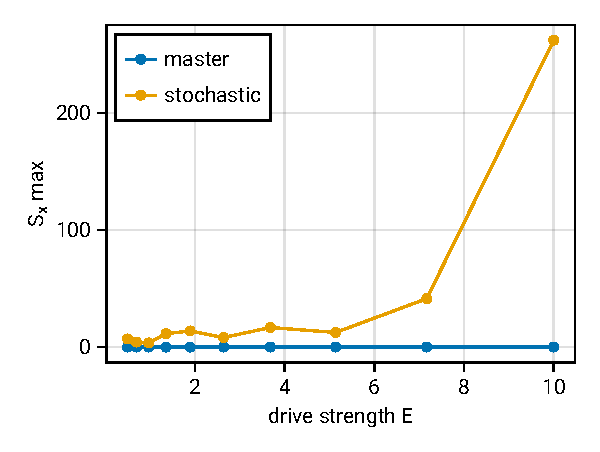
\includegraphics{figures/02 power.pdf}
	\\\small
	Took $\approx1$ min of compute time. Why is the SME so much slower? True Random Values?
\end{frame}

\begin{frame}{Expectation}
	\begin{columns}
		\column{.4\textwidth}
		$$S_x = S_x^\text{imp} + S_x^\text{ba} + S_x^\text{zpf}$$
		\small
		$S_x^\text{imp} \propto P^{-1} \omega^0$: Imprecision / Shot noise\\
		$S_x^\text{ba} \propto P$: Back action\\
		$S_x^\text{zpf}$: Zero Point Fluctuation

		\column{.6\textwidth}
		\centering
		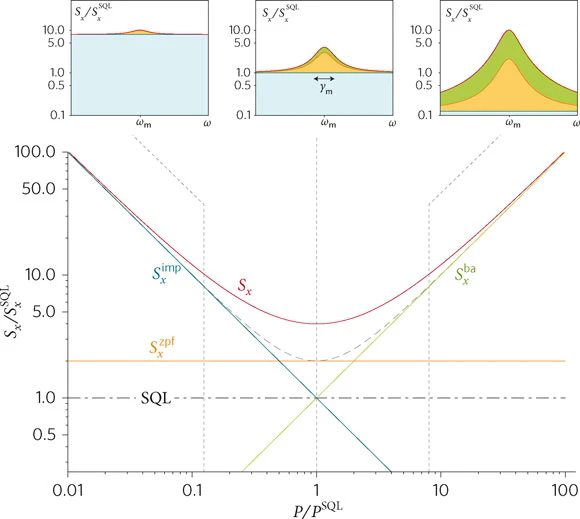
\includegraphics[width=\textwidth]{figures/Fig 1.png}
	\end{columns}
	\customcite[Fig. 1]{teufel_nanomechanical_2009}
\end{frame}

\begin{frame}{Uncerstanding $S_\text{det}(\omega, P_\text{in})$}
	\begin{columns}
		\column{.5\textwidth}
		Where is the power dependence?
		$$
		\overline S_\text{det}(\omega)
		= \frac{1}{8 \eta \Gamma |C_\text{eff}|}
		+ 2 \Gamma |\chi(\omega)|^2 |C_\text{eff}|
		$$
		$C_\text{eff}(\omega) = \frac{4 g^2}{\kappa \Gamma(1-2 i\omega /\kappa)^2}$\\
		$\chi(\omega) = \frac{\Omega}{\Omega^2 - \omega^2 - i\omega\gamma}$ \\
		$\eta$: Detection efficiency\\
		$\Gamma = \gamma$: Damping of oscillator\\
		
		\tiny 
		$$
		\overline S_\text{det}(\omega)
		= \frac{\kappa\Gamma |1-2i\omega/\kappa|}{8 \eta \Gamma 4 g^2}
		+ 2 \Gamma \frac{\Omega^2}{|\Omega^2-\omega^2-i\omega\gamma|^2}
		\frac{4 g^2}{\kappa \Gamma(1-2 i\omega /\kappa)^2}
		$$
		
		\customcite[eq. 3.51]{bowen_quantum_2015}

		\column{.5\textwidth}
		\small\centering
		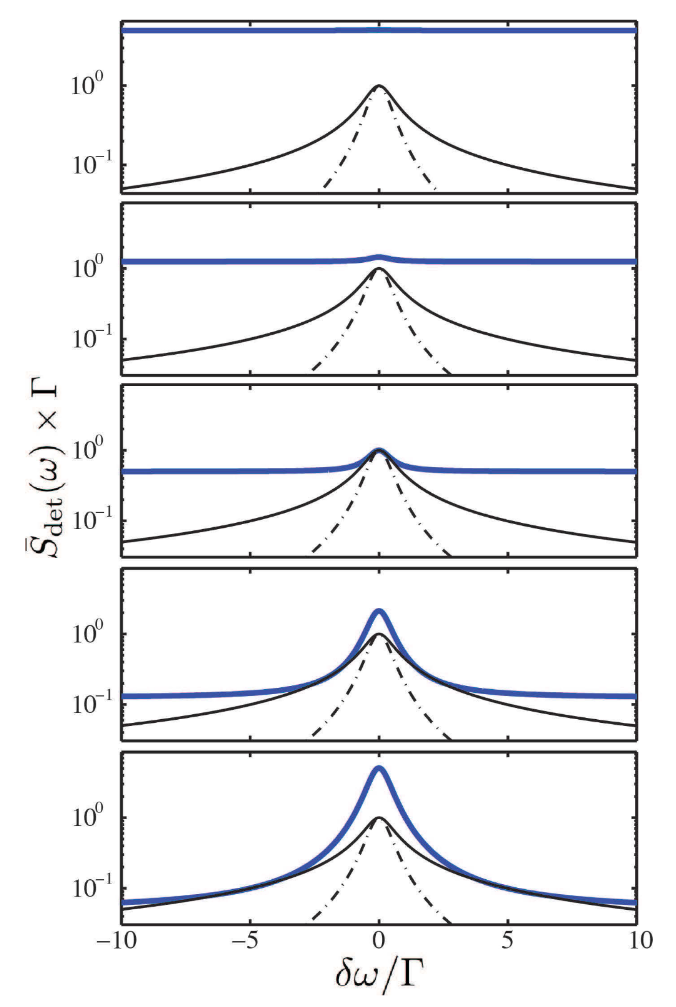
\includegraphics[width=\textwidth]{figures/3.5.png}
		$P/P^\text{SQL} = \{0.1, 0.4, 1, 4, 10\}$
		\customcite[Fig. 3.5]{bowen_quantum_2015}

	\end{columns}
\end{frame}

\begin{frame}
	\centering
	Looking for a source that derives $S_\text{det}(\omega, P)$?\\
\end{frame}

\end{document}